% !Mode:: "TeX:UTF-8"
% !TEX root = ..\paper.tex
\chapter{计算实验}
\section{实验结果与原始调度结果对比分析}
原始调度方案中,订单$1-4$安排入流水线$1$,$5-8$入流水线$2$以此类推,并根据EDD 规则进行调度安排,在决策参数$\lambda_1 = 0.6, \lambda_2 = 0.4$的环境下,分别采用Cyc -- ATC 算法、Cyc -- Tabu 算法和Vtr -- Tabu 算法求解结果,并与原始调度相比较,结果如\reft{tab:resultexample20}所示。
\begin{table}[h!]
  \centering
  \label{tab:resultmodel1}\caption{订单量$n = 20$的模型1 原始调度结果与$3$种算法求解结果}
    \begin{tabular}{cccl}
    \toprule
    算法    & 目标函数值($G$) & \multicolumn{2}{c}{流水线调度安排} \\
    \midrule
    \multirow{5}[2]{*}{原始调度} & \multirow{5}[2]{*}{$9312$} & $1$
        &  $\xymatrix{4 \ar[r] & 3 \ar[r] & 1 \ar[r] & 2}$\\
         &        & $2$     &  $\xymatrix{5 \ar[r] & 7 \ar[r]& 6 \ar [r]& 8}$\\
         &        & $3$     &  $\xymatrix{12 \ar[r] & 10 \ar[r] & 11 \ar[r] & 9}$\\
         &        & $4$     &  $\xymatrix{16 \ar[r] & 13 \ar[r]& 15 \ar[r] & 14}$\\
         &        & $5$     &  $\xymatrix{19 \ar[r] &18 \ar[r] & 17 \ar[r] &20}$\\
      \hline
    \multirow{5}[2]{*}{Cyc -- ATC} & \multirow{5}[2]{*}{$3978.8$} & $1$     &$\xymatrix{10 \ar[r] & 18 \ar[r] & 14 \ar[r] & 6}$\\
          &       & $2$     &  $\xymatrix{11 \ar[r] & 7 \ar[r] & 2}$\\
          &       & $3$     &  $\xymatrix{16 \ar[r] & 15 \ar[r] & 13 \ar[r] & 9}$\\
          &       & $4$     &  $\xymatrix{4 \ar[r] & 8 \ar[r] & 17 \ar[r] & 12 \ar[r]&20}$\\
          &       & $5$     &  $\xymatrix{5 \ar[r] & 1 \ar[r] & 3 \ar[r] & 19}$\\
     \hline
    \multirow{5}[2]{*}{Cyc -- Tabu} & \multirow{5}[2]{*}{$3478.8$} & $1$     &  $\xymatrix{10 \ar[r] & 6 \ar[r] & 18 \ar[r] & 14}$\\
          &       & $2$     & $\xymatrix{7 \ar[r] & 11 \ar[r] & 20 \ar[r] & 2}$ \\
          &       & $3$     &  $\xymatrix{9 \ar[r] & 13 \ar[r] & 16 \ar[r] & 15}$\\
          &       & $4$     &  $\xymatrix{4 \ar[r] & 8 \ar[r] & 17 \ar[r] & 12}$\\
          &       & $5$     &  $\xymatrix{5 \ar[r] & 19 \ar[r] & 1 \ar[r] & 3}$\\
       \hline
    \multirow{5}[2]{*}{Vtr -- Tabu} & \multirow{5}[2]{*}{$3329.2$} & $1$     &  $\xymatrix{10 \ar[r] & 20 \ar[r] & 18 \ar[r] & 2}$\\
          &       & $2$     & $\xymatrix{7 \ar[r] & 11 \ar[r] & 14 }$ \\
          &       & $3$     &  $\xymatrix{9 \ar[r] & 13 \ar[r] & 16 \ar[r] & 15\ar[r]&6}$\\
          &       & $4$     &  $\xymatrix{4\ar[r] & 8 \ar[r] & 3 \ar[r] & 12}$\\
          &       & $5$     &  $\xymatrix{5 \ar[r] & 19 \ar[r] & 1 \ar[r] & 17}$\\
    \bottomrule
    \end{tabular}
  \label{tab:resultexample20}
\end{table}
\section{模型1 求解结果与分析}
以$m = 6, n = 200$ 为例,决策参数和目标函数值的关系如\reff{fig:decisionvsG}所示。
\begin{figure}
\centering
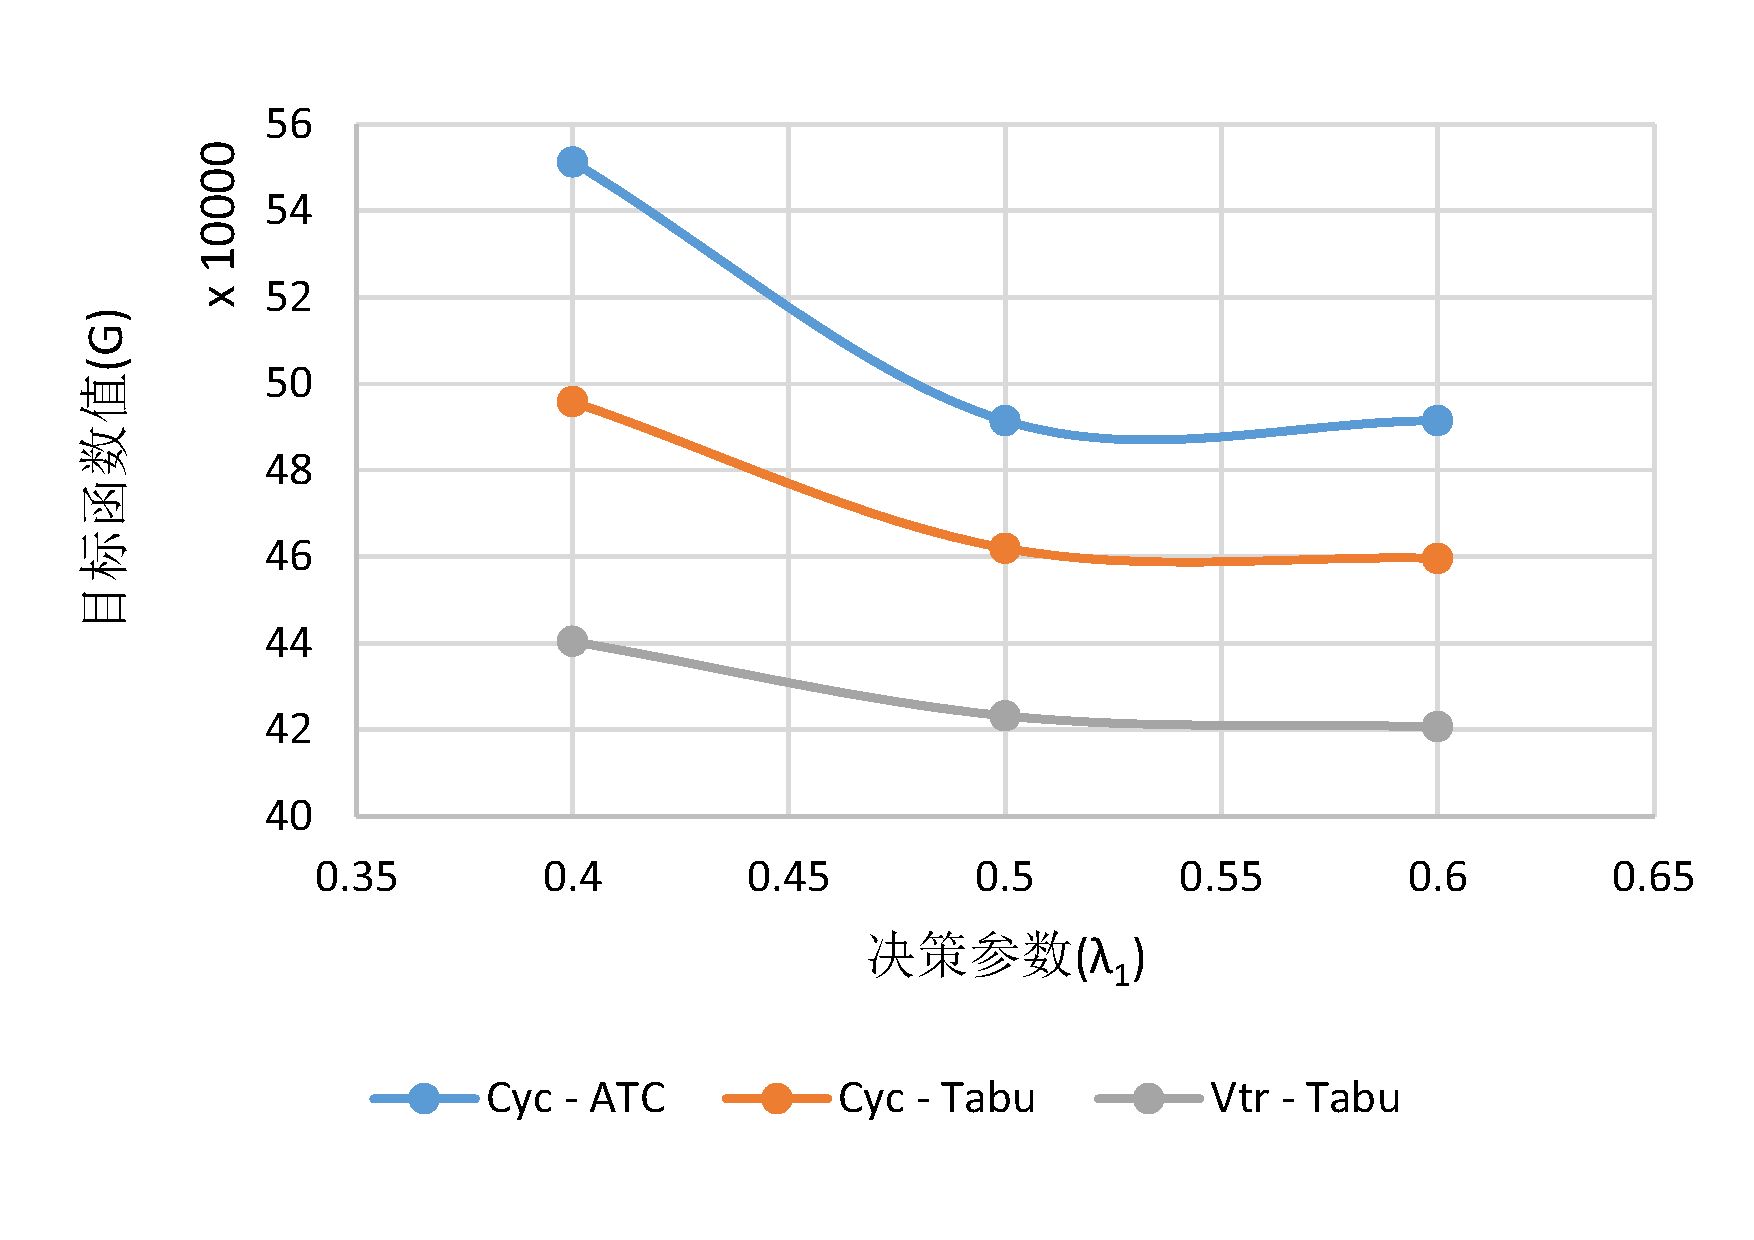
\includegraphics[height = 7cm, angle = -90]{lambda.pdf}
\caption{决策参数和目标函数值关系示例}\label{fig:decisionvsG}
\end{figure}
可以看出,随着决策参数$\lambda_1$的增大,即更为看重工期目标,三个算法所得的目标值都减少,说明模型1 适用于强调工期的调度问题。其他的决策环境下,所得结论基本一致。
问题规模较小的时候,Vrt -- Tabu 算法对解的改进效果比较明显。并且随着决策参数$\lambda_1$的增大,Vtr -- Tabu 算法的改进效果也越为明显,也就是说,如果决策者对交付期较为重视的话,选择Vtr -- Tabu 算法来求解调度方案是比较好的。
\section{模型2 求解结果及分析}
在决策参数$\lambda_1 = 0.5$ 的环境下,$3$种算法所得不同流水线数所得调度的流水线均衡率如\reff{fig:linenumbervsrate}所示。
\begin{figure}[h]
\centering
\subfloat[$m = 5$]{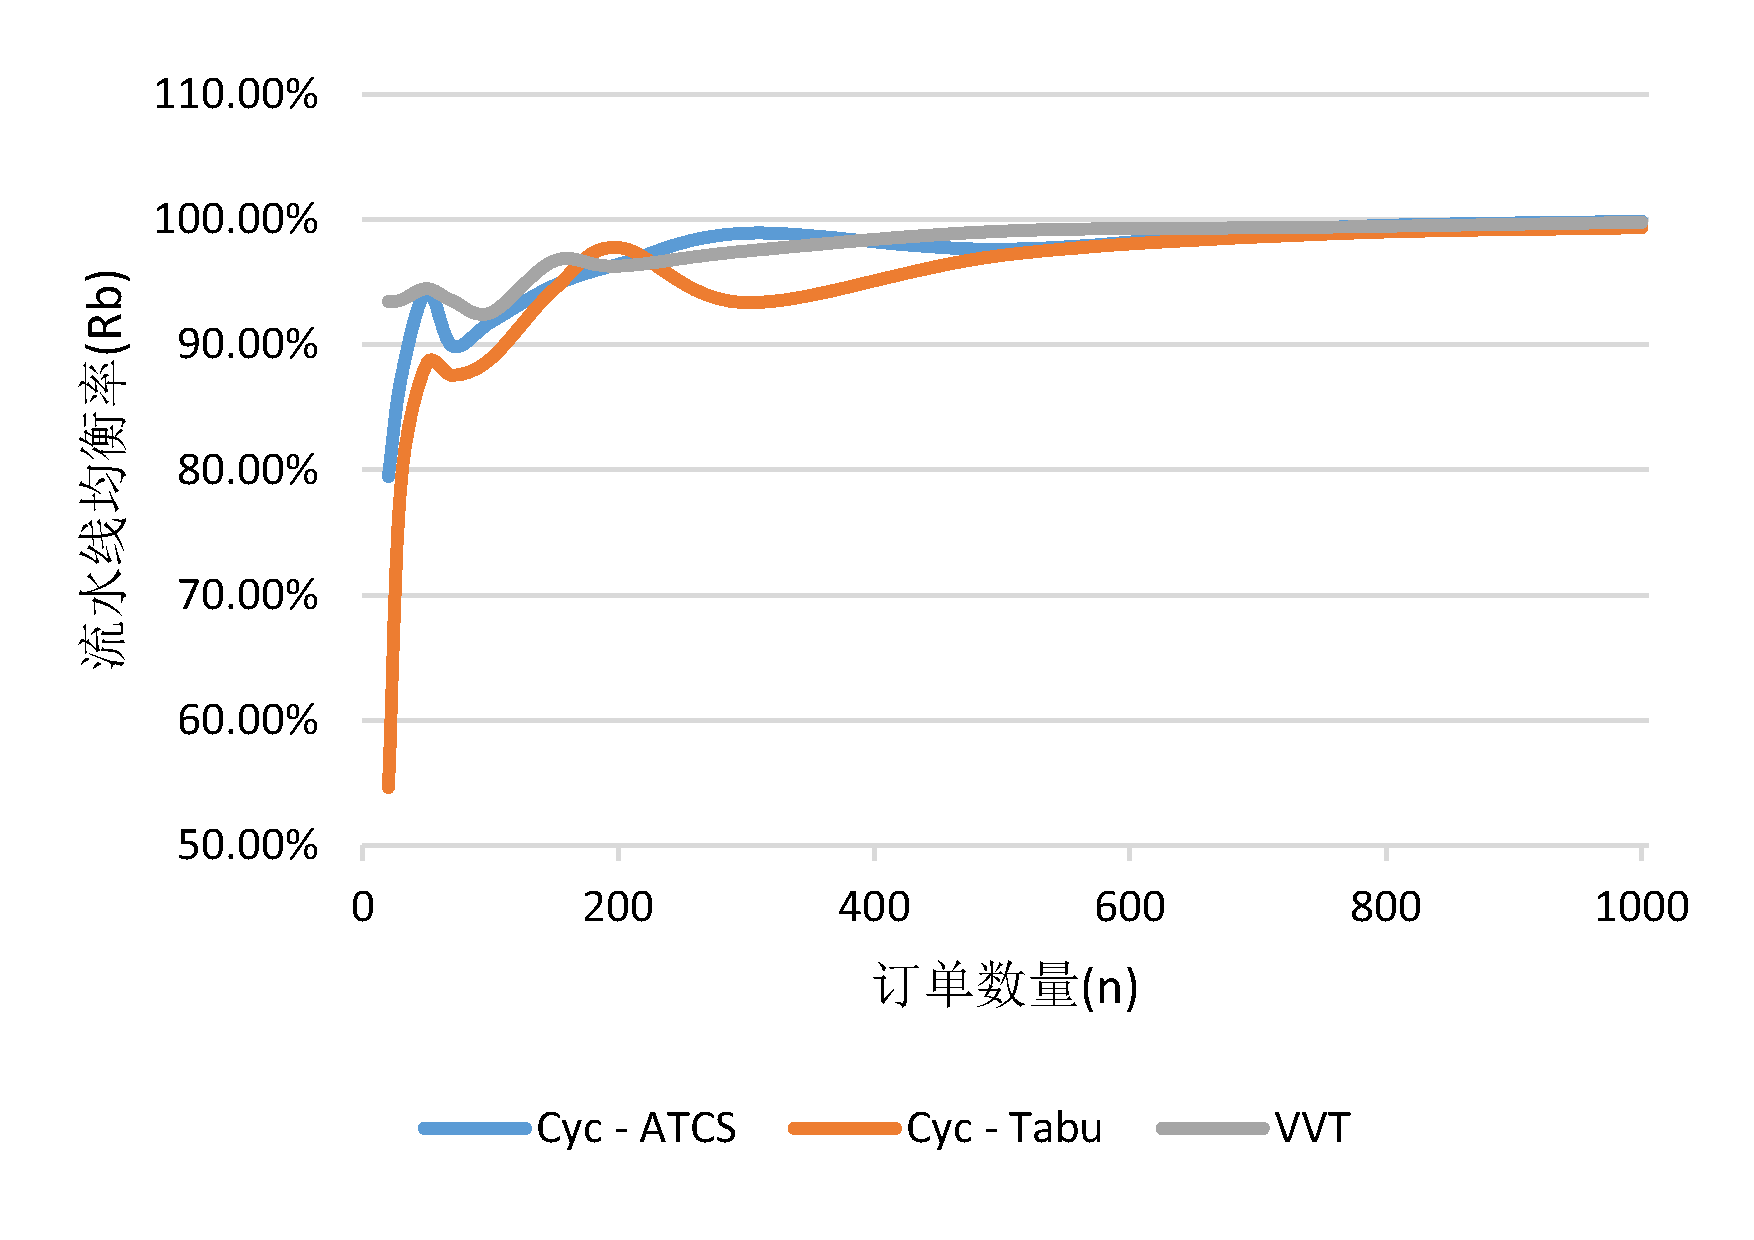
\includegraphics[height = 5.6cm,angle = -90]{rb_05_5.pdf}}
\subfloat[$m = 6$]{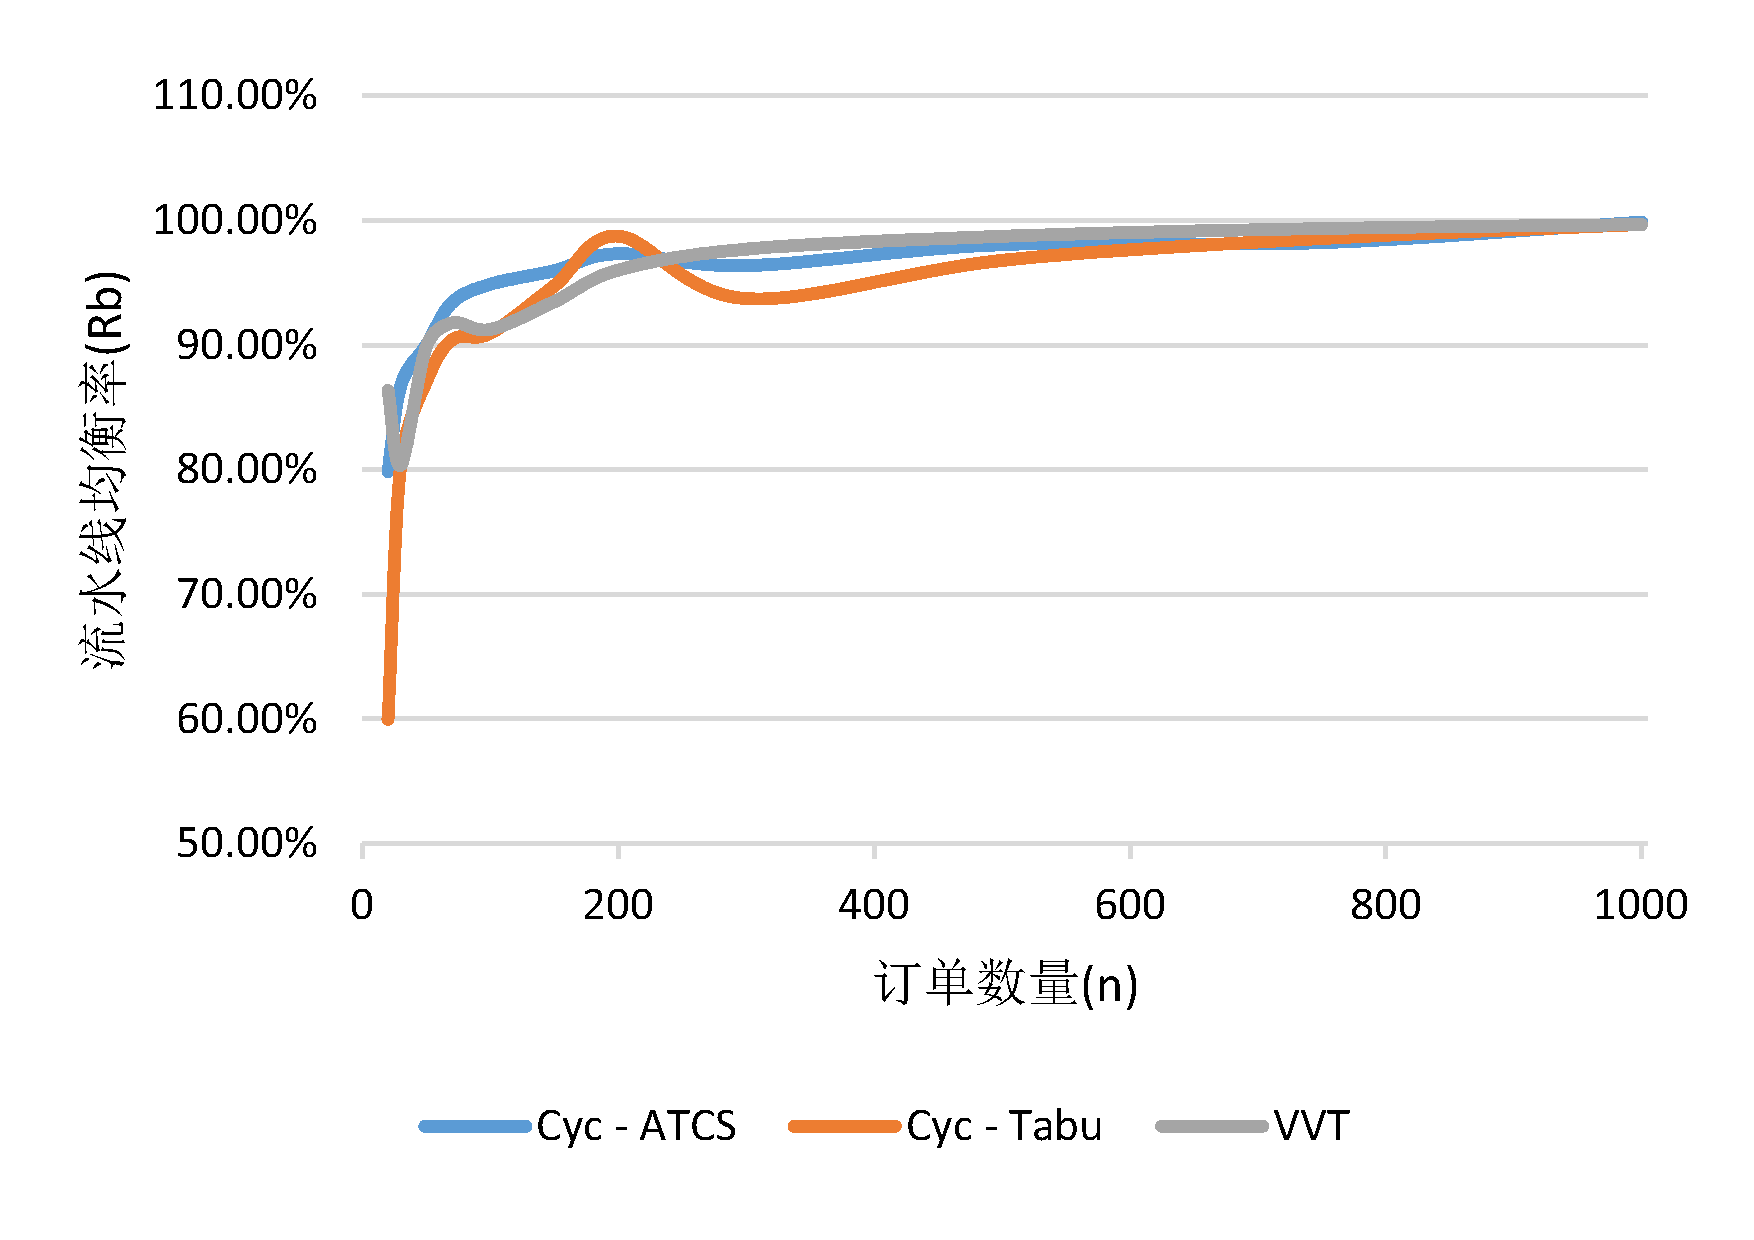
\includegraphics[height = 5.6cm,angle = -90]{rb_05_6.pdf}}
\subfloat[$m = 7$]{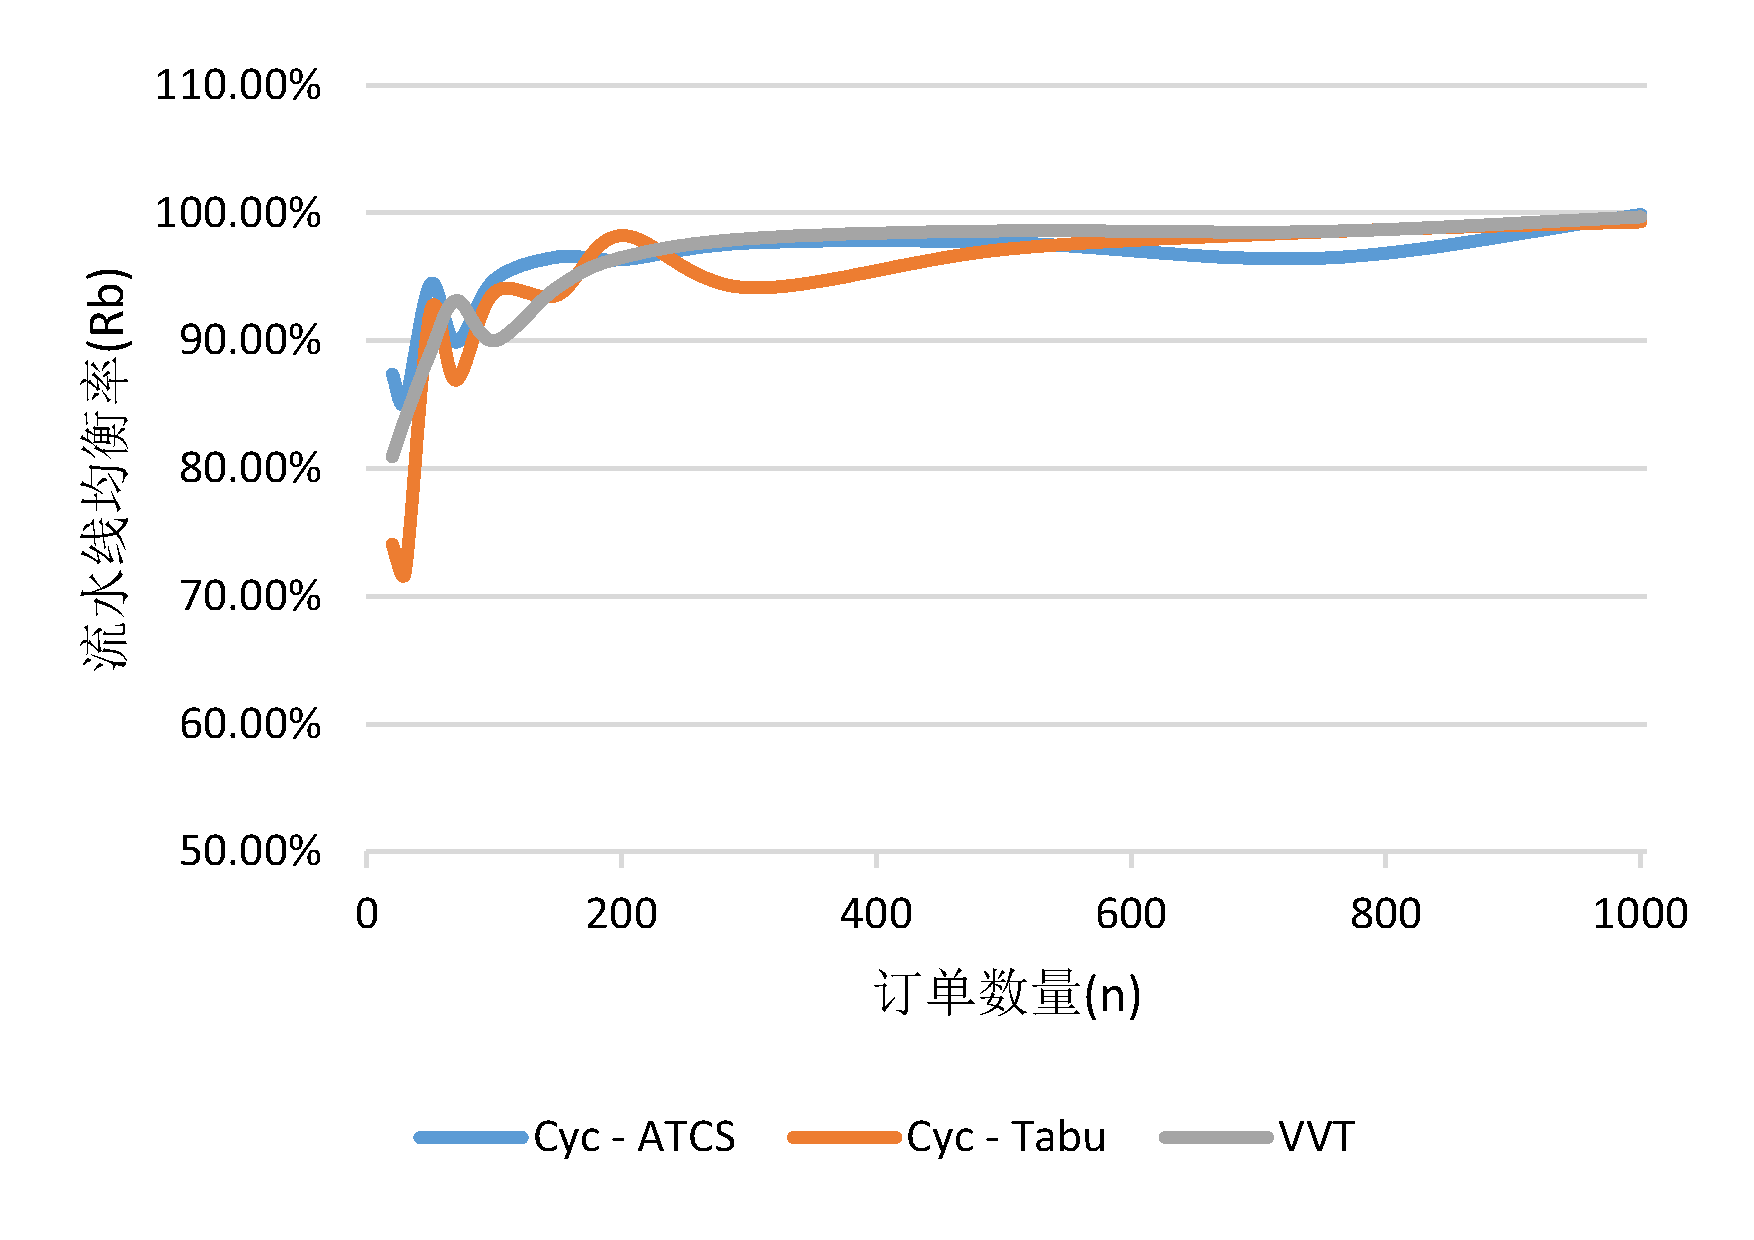
\includegraphics[height = 5.6cm,angle = -90]{rb_05_7.pdf}}
\caption{不同流水线数量和流水线均衡率关系}\label{fig:linenumbervsrate}
\end{figure}

可以看出,$3$个算法中,VVT 算法所得的流水线均衡率随订单数量的增加最为稳定,始终可以保持一个较高的水平,而Cyc -- Tabu 算法则会有较大波动。随着订单数量增加,各算法所得的流水线均衡率都大约成对数趋势增加趋向于$100\%$,一般在$n = 500$左右稳定在较高值,这十分符合常理,并且随着流水线数量的增加,各算法的稳定点都前移($n$减少的方向)。
随着流水线数量$m$的增加,Cyc -- Tabu 算法和VVT 对解的改进效果和Cyc -- ATCS 相差不大(除个别情况外),但VVT 算法所得结果较为稳定。

流水线$m = 6$ 的环境下,$3$种算法所得不同决策环境下调度的流水线均衡率如\reff{fig:decisionvsrate}所示。
\begin{figure}
\centering
\subfloat[$\lambda_1= 0.4$]{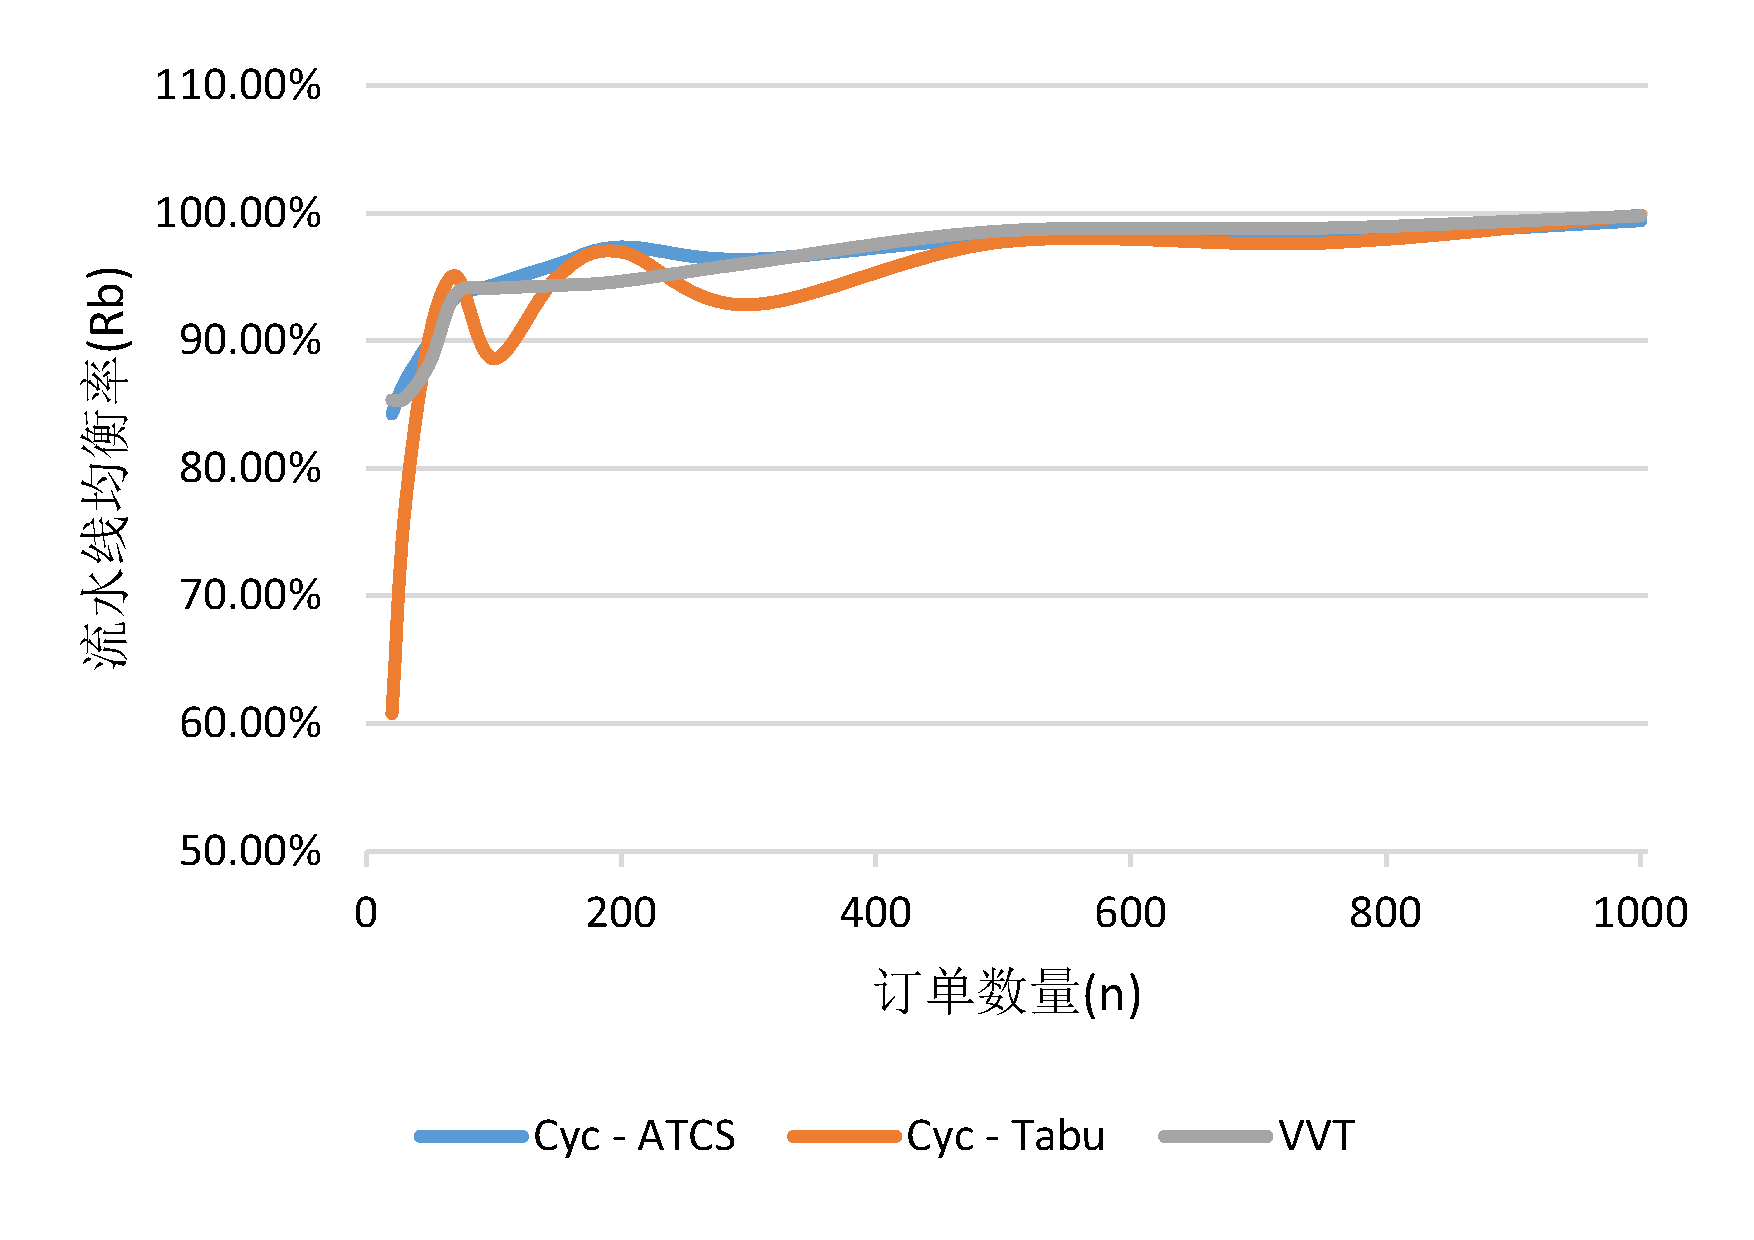
\includegraphics[height = 5.6cm,angle = -90]{rb_04_6.pdf}}
\subfloat[$\lambda_1= 0.6$]{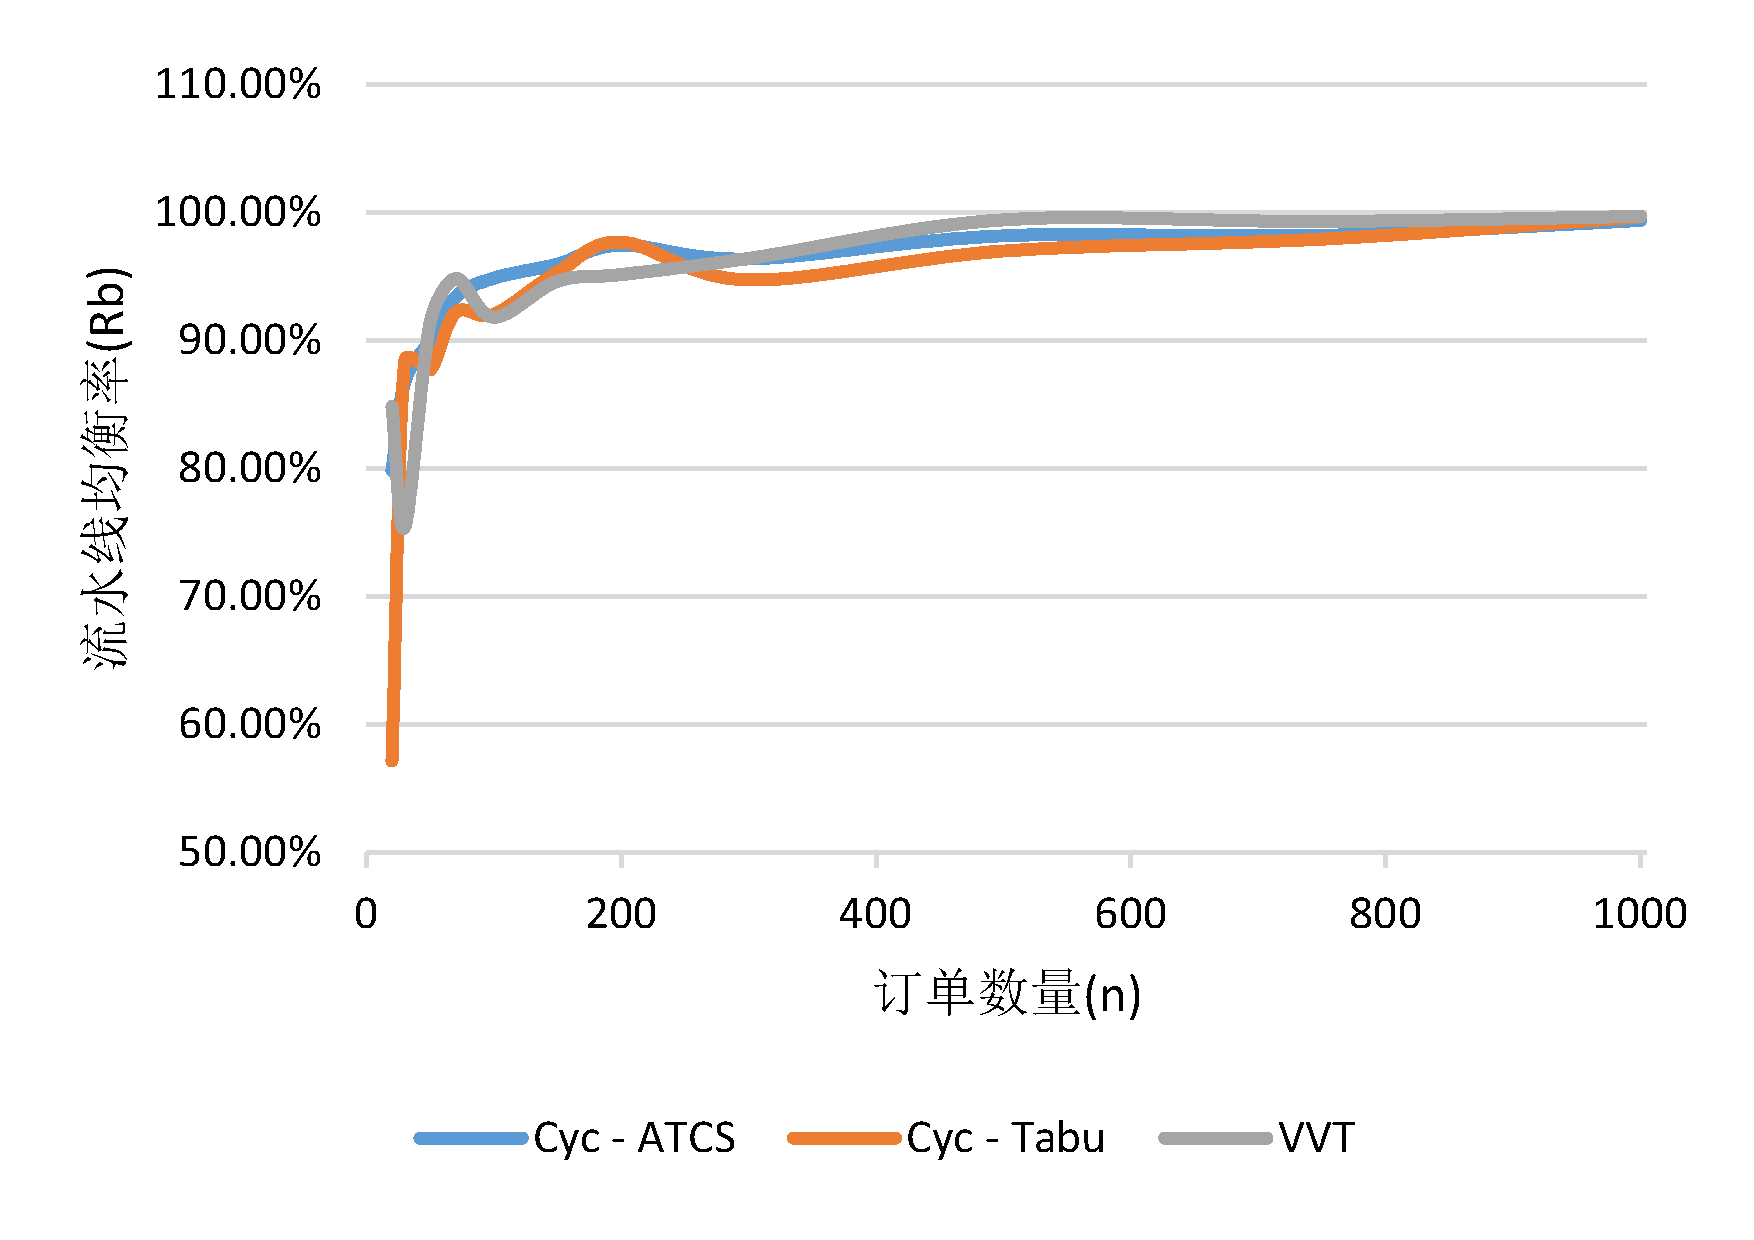
\includegraphics[height = 5.6cm,angle = -90]{rb_06_6.pdf}}
\caption{决策环境和流水线均衡率关系}\label{fig:decisionvsrate}
\end{figure}

与流水线均衡率分析类似,不同决策环境下,VVT 算法所得的流水线均衡率随订单数量的增加最为稳定,始终可以保持一个较高的水平,而Cyc -- Tabu 算法所得结果由较大波动,而且随着决策参数$\lambda_1$的增加,即大工期目标的重要性,各算法都会逐渐产生较为稳定的流水线均衡率,并且稳定点都前移。说明模型2 的设计是符合工期要求的,并且能明显提高流水线生产均衡率。

